
The performance of the distributed algorithms are studied in this section by comparing with the centralized algorithms. The performance is compared using the total number of backlogged packets after each \ac{SCA} update points. Fig. \ref{fig-d-1} compares the performance of the algorithms for the system configuration \me{\lbrace N,N_B,K,N_R \rbrace = \lbrace 3,2,8,1 \rbrace} with \me{N_T = 4} transmit antennas at the \acp{BS}. Each \ac{BS} serves \me{|\mc{U}_b| = 4} users in a coordinated manner to reduce the total number of backlogged packets at each \ac{BS}. As pointed out in Section \ref{sec-4}, the performance and the convergence speed of the distributed algorithms are susceptible to the choice of the step size used in the subgradient update. Since the interference values are fixed for local subproblem in the primal approach, it may lead to infeasible solutions if the initial or any intermediate update using \eqref{primal-sg-update} is not valid.

The Fig. \ref{fig-d-1} plots the performance of the primal and the \ac{ADMM} solutions for the \ac{JSFRA} scheme using \ac{SCA} and by \ac{MSE} relaxation at each \ac{SCA} points. In between the \ac{SCA} updates, the primal or the \ac{ADMM} schemes are performed for \me{J_{\max} = 20} iterations by exchanging either the fixed interference variables in the primal approach or the dual variables in the \ac{ADMM} scheme. It can be seen from Fig. \ref{fig-d-1} that the distributed algorithms approaches the centralized performance by exchanging minimal information between the coordinating \acp{BS}.
\begin{figure*}
\centering
\subfloat[][System \me{\lbrace N,N_B,K,N_R \rbrace = \lbrace 3,2,8,1 \rbrace}]{
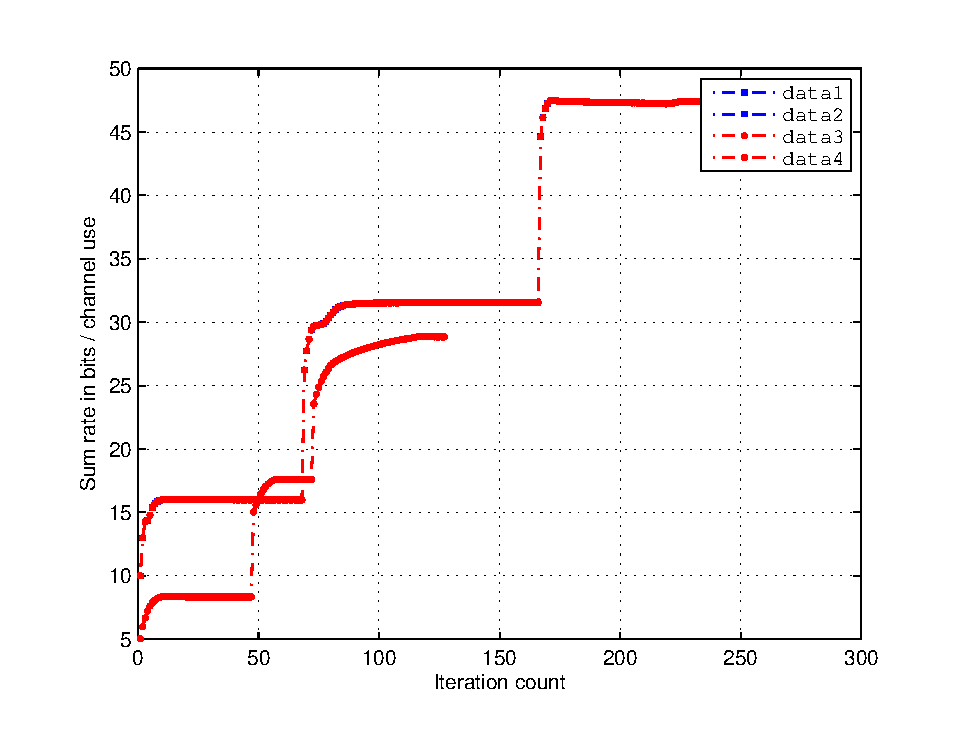
\includegraphics[width=0.48\textwidth]{fig-3}
\label{fig-d-1}
}
\hfill
\subfloat[][System \me{\lbrace N,N_B,K,N_R \rbrace = \lbrace 6,3,12,2 \rbrace}]{
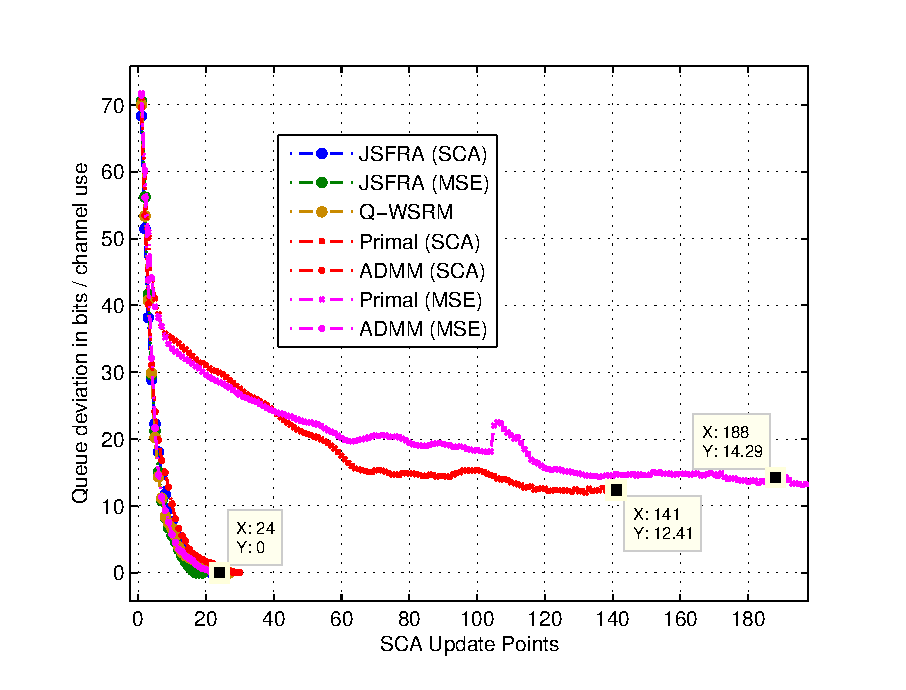
\includegraphics[width=0.48\textwidth]{fig-5}
\label{fig-d-2}
}
\caption{Number of backlogged packets at each \ac{SCA} points}
\label{fig-d}
\end{figure*}

In Fig. \ref{fig-d-2}, the performance of the distributed algorithms are studied for \me{K = 12} users utilizing \me{N = 6} sub-channels. The system considers \me{N_B = 3} \acp{BS}, each having \me{N_T = 4} transmit antennas serving \me{|\mc{U}_b| = 4} users equipped with \me{N_R = 2} antennas respectively. The users are assumed to be scattered over the cell boundary experiencing the path loss following the uniform distribution between \me{[0,-6]} dB. The performance of the algorithms are similar to the \me{N_B = 2} \ac{BS} scenario discussed earlier.

Fig. \ref{fig-d-2} plots the performance of the centralized and the distributed algorithms at each \ac{SCA} update. In case of the distributed algorithms, in between each \ac{SCA} update, the primal or the \ac{ADMM} exchanges are performed for \me{J_{\max} = 20} iterations. In practice, \me{J_{\max} = 1} can be set to perform the \ac{SCA} update, \ac{ADMM} or primal update, and the receive beamformers \me{\mvec{W}{k,n}} update at the same instant. The data tips are used to highlight the convergent points of various algorithms. The performance of the \ac{JSFRA} schemes using the primal decomposition are notably inferior compared to the \ac{ADMM} approach for the same schemes. It is mainly attributed to the difficulty in selecting the step size for the system employing \me{N_B \geq 3} \acp{BS}.
% \begin{figure*}
% \centering
% \begin{subfigure}{0.49\textwidth}
% 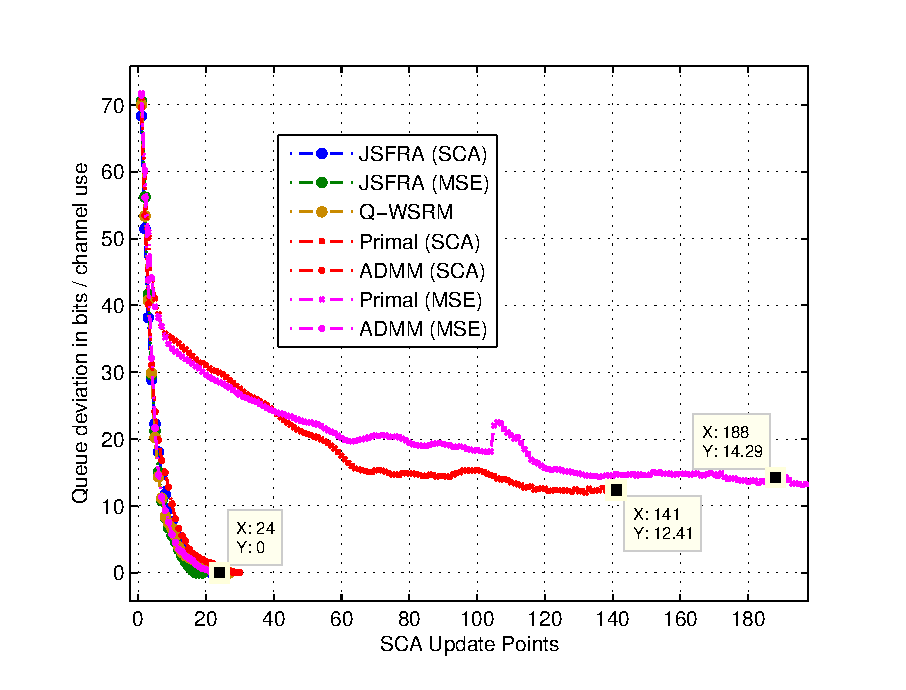
\includegraphics[width=\textwidth]{fig-5}
% \caption{Queue deviation}
% \end{subfigure}
% \hfill
% \begin{subfigure}{0.49\textwidth}
% 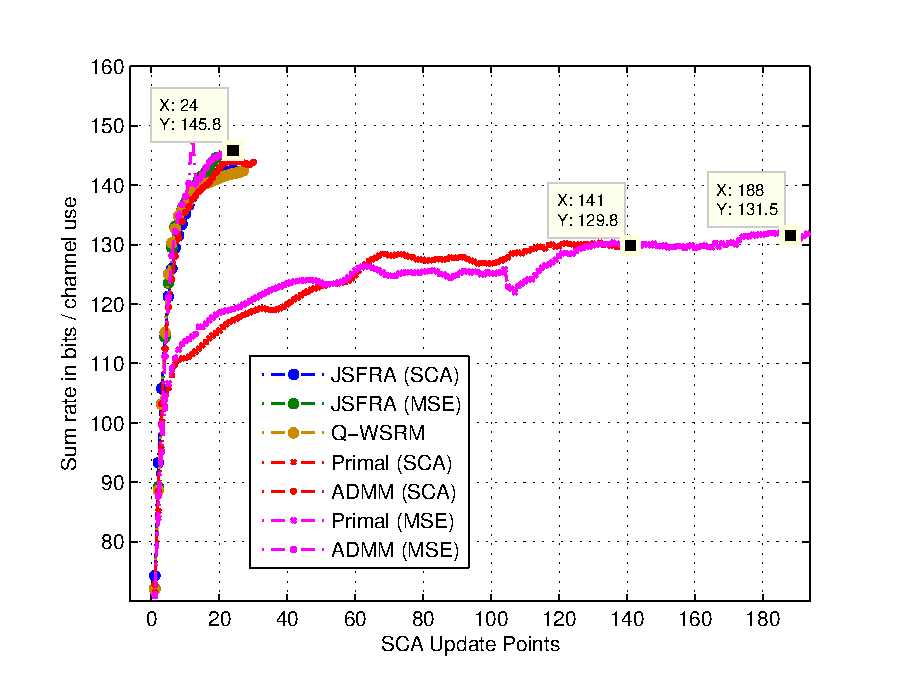
\includegraphics[width=\textwidth]{fig-6}
% \caption{Sum rate performance}
% \end{subfigure}
% \caption{Convergence plot for \me{\lbrace N,N_B,K,N_R \rbrace = \lbrace 6,3,12,2 \rbrace} model}
% \label{fig-d-2}
% \end{figure*}

Fig. \ref{fig-d-3.1} compares the performances of the centralized algorithm based on the \ac{MSE} reformulation with the iterative approach proposed in Section \ref{sec-4.3} based on solving the \ac{KKT} conditions. In Fig. \ref{fig-d-3.1}, the plots are compared by the surplus number of backlogged packets at the end of each iteration or the \ac{SCA} update point. Fig. \ref{fig-d-3.1} shows that the \me{\ell_1} norm for \ac{JSFRA} scheme provides better performance over rest of the schemes due to its greedy objective. The \ac{KKT} approach for \me{\ell_1} norm is not defined due to the non-differentiability of the objective as discussed in the Section \ref{sec-4.3}, thereby performs the worst of all other approaches. The heuristic method used in the figure is obtained by forcing the dual variable \me{\sigma_{l,k,n}} in \eqref{kkt-mse-4.2} to \me{0} when the queue deviation is negative \me{Q_k - t_k < 0}, if not, then it will be the same as in \eqref{kkt-mse-4.2}. The additional condition can be justified due to the dropping of absolute value operator from the objective. It can be seen that the heuristic method oscillates near the optimal point with the deviation determined by the factor \me{\rho} used in \eqref{kkt-mse-4.1}.
\begin{figure}
\centering
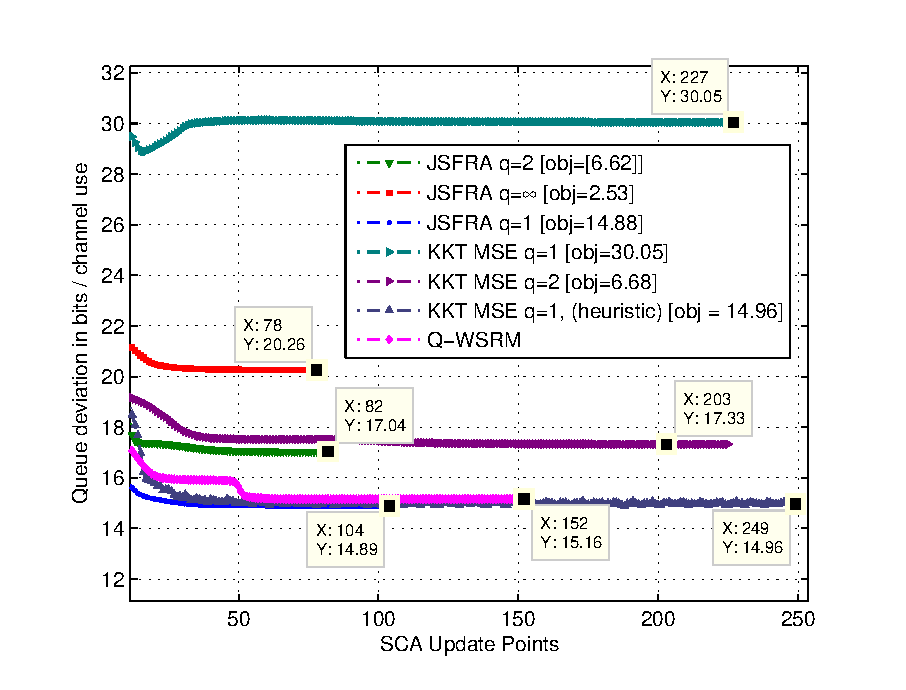
\includegraphics[width=\columnwidth]{fig-9-2}
\caption{Convergence plot for \me{\lbrace N,N_B,K,N_R \rbrace = \lbrace 5,2,8,1 \rbrace} model}
\label{fig-d-3.1}
\end{figure}

The objective values are mentioned in the legend for all the schemes, since the objective of \me{\ell_2} norm is not the same as \me{\ell_1} norm, which is used for the plot. The \me{\ell_2} norm for the \ac{JSFRA} and the \ac{KKT} based approach achieves nearly the same objective value of \me{6.62} but different \me{\chi}, since the dual variables \me{\alpha_{l,k,n}} and \me{\sigma_{l,k,n}} are not iterated until convergence between each \ac{SCA} steps in the \ac{KKT} approach. In the simulation, we update all the variables at each iteration due to the practical issues in the signaling between the \acp{BS}. Fig. \ref{fig-d-3.1} also compares the effect of dropping the squared rate variable from the objective in the \ac{Q-WSRME} scheme compared to the \me{\ell_2} norm which includes it. By dropping the squared rate variable, the \ac{Q-WSRME} scheme minimizes the number of queued packets in a prioritized manner based on the respective queues. On contrary, the \me{\ell_2} norm allocate rates to the users with the higher number of queued packets before addressing the users with the smaller number of queued packets.


